\documentclass[12pt]{article}
\usepackage{setspace}
\usepackage{amsmath}
\usepackage[utf8]{inputenc}
\usepackage{pgfplots}
\pgfplotsset{compat=1.18}
\oddsidemargin=0.0in
\evensidemargin=0.0in
\textwidth=6.3in
\headheight=0.0in
\topmargin=0.0in
\textheight=8.9in
\title{Minimising Portfolio Loss in Portfolio Construction}
%\date{16-12-2021}
\author{Colin M. Smith BITA Risk}
\begin{document}
\maketitle
\tableofcontents
\pagebreak
\doublespacing
\section{Introduction}
This document attempts to show how to use portfolio loss minimisation in the
portfolio enhancement process. We start by defining $Loss$ and compare
the predicted changes to a portfolio achieved by adopting minimal $Loss$ against minimal $Risk$. Then we indicate how 
$Loss$ minimisation could replace or augment $Risk$ minimisation in the portfolio enhancement process.
Finally a more tractable $`$Gain Loss with a twist' is described. We propose using
the factor model to find predicted asset return series and use these to define predicted $Loss$. 
By minimising portfolio $predicted\ Loss$ in the enhancement, we should get a faster calculation since 
the predicted 
power of the risk model can be delivered by as few as three months of data.

\section{Definition of Portfolio Gain and Loss}
Over the history of a portfolio it is usual to monitor its return each period and the returns of the underlying assets.
From one period  to the next, the portfolio's return will change and to characterise this change we can define its gain or loss.
To make the gain and loss a little more configurable we define 
gain $G$ and loss $L$ with respect to a target return $R$ which could be positive or negative.
Suppose the portfolio return series at time $t$ is $r(t)$ then
\begin{eqnarray}
    G = \sum_t {\textbf{ max} }(r(t) - R,0)
\end{eqnarray}
\begin{eqnarray}
    L = \sum_t {\textbf{ max} }(R-r(t),0)
\end{eqnarray}
This means that in period $t$, if $R-r(t) > 0$ there is a loss, and if $R-r(t) < 0$ there is a gain.
If we define a loss period as one for which $R-r(t) > 0$,
\begin{eqnarray}
  {\rm Total\ Loss},\ L= \sum_{t\ \in\ \rm loss\ periods} R-r(t)
\end{eqnarray}
$G$ and $L$ are both non-negative and
\begin{eqnarray}
 {\rm   total\ portfolio\ return}= G - L + RT
\end{eqnarray}

If there are $n$ assets in the portfolio and each asset $i$
has a weight $w_i$ and a return series $s_i (t)$ then
\begin{eqnarray}
    r(t) = \sum_{i=1}^{n} w_i s_i(t)
\end{eqnarray}
The expected return for asset $i$, $\alpha_i$ may be calculated from
mean\footnote{We calculate $\alpha$ using arithmetic mean. $\alpha_i$ and target rate are values per-period.} 
return of $s_i(t)$.
\begin{eqnarray}
    \alpha_i =  \frac{1}{T}\sum_{t=1}^{T} s_i(t)
\end{eqnarray}
where $T$ is the number of periods.

\section{Comparison of Optimal Portfolio Weights in Risk and Loss Minimisation}

Following the standard portfolio construction methods, the practioner seeks to find a portfolio that 
will give a certain amount of return for small risk. Instead of minimising risk, we could find the 
lowest possible loss. For illustration purposes, consider a small portfolio of 9 assets
for which we have a return series for each asset.
The following barchart shows the outcome weights for two portfolio optimisations. There are $423$ data periods in the
return series. In both optimisations\footnote{The weights are constrained to satisfy the budget $\sum w_i = 1$} the return is 
constrained to $0.005$ and the target rate per period is $0.0004$; the blue bars show the weights
for mininum risk ($0.058$) which gives a portfolio with total loss of $1.34$ and the pink bars show
the weights for minimum total loss ($1.15$) with a risk of $0.085$. The risk quoted is historic risk and is 
calculated directly as the standard deviation of the portfolio return series. We don't annualise risk and return or 
express them as percentage values here.
\break
\break
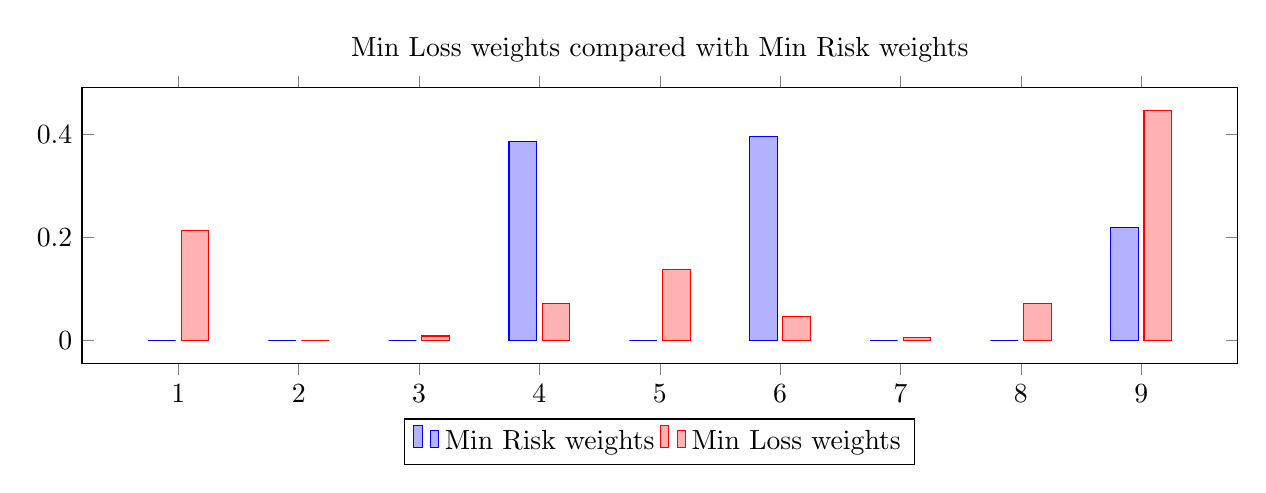
\begin{tikzpicture}
    \begin{axis}
        [title={Min Loss weights compared with Min Risk weights},
        ybar,height=2in,width=6.4in, symbolic x coords={1,2,3,4,5,6,7,8,9},
        legend style={at={(0.5,-0.2)},        anchor=north,legend columns=-1}]
        \addplot coordinates {(1,0)
        (2,0) 
        (3,0)
        (4,0.3854726513396513)
        (5,0)
        (6,0.3950537500804109)
        (7,0)
        (8,0)
        (9,0.21947359857993776)};
        \addplot coordinates {
            (1,0.2131871336385196)
            (2,0)
            (3,0.008529985052857314)
            (4,0.07179520200177866)
            (5,0.13819750244263093)
            (6,0.046937456187809756)
            (7,0.0047705423361060345)
            (8,0.07143877895977421)
            (9,0.4451433993805218)};
            \legend{Min Risk weights,Min Loss weights}
    \end{axis}
\end{tikzpicture}
\break
\break
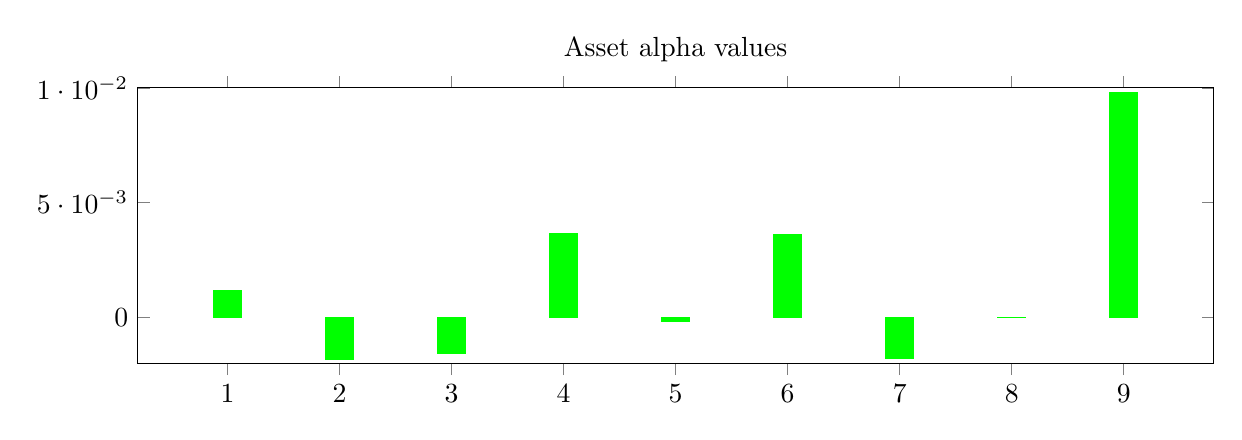
\begin{tikzpicture}
    \begin{axis}[title={Asset alpha values},
        ymin=-0.002,
        ymax=0.01,
        scaled y ticks=false,yticklabel style={/pgf/number format/1000 sep=},
        ybar,height=2in,width=6in,symbolic x coords={1,2,3,4,5,6,7,8,9}]
        \addplot coordinates{
            (1,0.0011707063636410724)
            (2,-0.0018399458749987034)
            (3,-0.001547403488527072)
            (4,0.003674758692542117)
            (5,-0.00016312751189371318)
            (6,0.003627629196094118)
            (7,-0.001805179090833558)
            (8,-0.000010932381824192851)
            (9,0.009797864161556428)}[color=green];
    \end{axis}
\end{tikzpicture}
\break
Notice that the $Loss$ minimising portfolio achieves its constrained return by putting most weight in the
asset with highest alpha, and uses a diverse selection of the other assets to make up the remaining 
return. It even chooses assets with negative alpha\footnote{This is a consequence of the budget constraint}. The $Risk$ minimising portfolio is less diverse and makes far less use of the asset with highest alpha.

If we just maximised return subject to the budget, the portfolio would have all weight in the last 
asset and the return would be $0.0098$.

\section{Minimising Loss in the Enhancements}
The portfolio enhancement process consists of a host of regulatory constraints and other constraints 
designed to improve portfolio expected return. It is necessary to control the uncertainty in the return usually 
by managing the risk.
A straightforward implementation of loss optimisation might be to replace the risk optimisation with loss minimisation.
Over the entire history the weights could be chosen to minimise total portfolio $Loss$.
This would require full asset return history to define $Loss$ and could 
result in a slow optimisation process since the amount of history\footnote{It would be possible 
to use a risk constraint as well but this would mean even longer execution time.} is so vast.  An advantage of
minimising $Loss$ over minimising $Risk$ is that the resulting weights are likely
to be more diversifing. Looking at the simple graph for 9 stocks in the previous section we see that
$Loss$ minimisation results in higher weight in the high alpha asset with many 
smaller changes in the other assets to get the lowest loss. ($Risk$ optimisation gives a less diverse
result and a lower weight in the high alpha asset). We conjecture from this that $Loss$ minimisation 
would make less impact on the strength of the factor premia terms, than $Risk$ minimisation although by definition it cannot
manage risk as well. This may not matter though; the difference in weight outcomes
highlights that the gains and losses in the optimisation are not symmetrically
distributed. ($Risk$ minimisation penalises gains and losses from the mean the same.) If they were, minimising $Loss$ would be very similar to minimising historic $Risk$, (although
we do impose our own asymmetricity by having a non-zero target rate.) It is important
to note that the factor premia must not be constrained too high, otherwise there is no scope 
for minimising $Loss$ (or $Risk$ either). In the example in the previous section 
if we had constrained the return to be $0.0098$ the only possible outcome has $100\%$ in 
the last asset.

The simple example explicitly contains an alpha constraint, but alpha as such does not need to 
be part of the optimisation. Instead of $`$alpha' we could insert $`$momentum' and include the momentum 
vector in the constraints instead of the alpha vector. We use alpha as a proxy for all 
possible constraints of interest.
\section{Minimising Modelled Loss}
The calculation outlined in the previous section might be thought of as $`$traditional gain loss'; it
minimises $historic\ loss$ subject to all of the portfolio constraints. Usually the risk in 
portfolio enhancement is modelled risk; it might be better to use $modelled\ loss$ here.

The risk model estimation process uses factor premia returns $p_{i}(t)$ in the regression
with asset returns. If there are $n_f$ factor premia, the modelled asset return $\hat{r}_{k}(t)$ for asset $k$ may be written
\begin{eqnarray}
    \hat{r}_{k}(t) = \sum_{i=1}^{i=n_f}\beta_{ki} p_{i}(t)
\end{eqnarray}
at time $t$, where $p_i$ is the i'th factor return and $\beta_{ki}$ is the usual factor loading matrix of regression coefficients.
This neglects the specific return which is not explained by the factors. The specific returns aren't of interest here because we want 
to maximise the effects due to just the factors. It is only necessary to include the factors which we expect 
to drive high returns.
Due to observed cycle conditions exhibited by the factors, a 3 month forecast window\footnote{One month is observed to be too short an estimation period.} of factor premia data may be enough
to get a good prediction of future return, so instead of incorporating the full history of
asset returns $r_k(t)$ in the optimisation it may be enough to use the modelled predictions
$\hat{r}_{k}(t)$ over a much reduced time horizon. The shorter the history for defining the
loss, the faster the optimisation, so there is a practical reason for this as well as
a theoretical one. Judging from the weights obtained in the simple 9 stock loss minimisation, we would expect 
that minimising the loss defined by $\hat{r}_{k}(t)$, subject to factor premia constraints, would favour mainly weights 
with high exposure to the factor premia together with diversifing weights that enable the lowest modelled loss.
\end{document}

